\documentclass[12pt,a4paper]{article}
\usepackage[utf8]{inputenc}
\usepackage{geometry}
\usepackage{graphicx}
\usepackage{amsmath}
\usepackage{hyperref}
\usepackage{titlesec}
\usepackage{changepage}
\usepackage{caption}
\usepackage{float}
\usepackage{booktabs}
\usepackage{hyperref}
\usepackage{tabularx}
\usepackage[numbers]{natbib} % Menambahkan paket natbib untuk referensi
\usepackage{setspace} % Untuk mengatur spasi antar baris

% Page layout
\geometry{top=1in, bottom=1in, left=1in, right=1in}

% Modify section and subsection font size to normal
\titleformat{\section}[hang]{\normalsize\bfseries}{\thesection}{1em}{}
\titleformat{\subsection}[hang]{\normalsize\bfseries}{\thesubsection}{1em}{}

% Hanging indent for references
\setlength{\bibsep}{1em} % Mengatur jarak antar entri referensi
\setlength{\bibhang}{2em} % Mengatur indentasi menggantung untuk referensi

\begin{document}

% Title
\begin{titlepage}
    \centering
    {\Large\textbf{Deep Learning Course \\ Final Project Report}\par} % Judul
    \vspace{2cm} % Jarak antara judul dan logo
    \includegraphics[width=0.5\linewidth]{Logo Terbaru.png}\par % Logo
    \vspace{2cm} % Jarak antara logo dan nama
    {\large
    Khaerurrozikin(H071221069)\\ 
    Andi Ahmad Salwan (H071221048)\\ 
    Muhammad Aditya Permana (H071221063)\par}
    \vspace{1cm} % Jarak antara nama dan tanggal
    {\large\today\par} % Tanggal
\end{titlepage}

\normalsize  % Set the text size to normal for the entire document
\tableofcontents
\newpage

% 1. Introduction
\section{INTRODUCTION}
\subsection{Latar Belakang }
\begin{adjustwidth}{3em}{0pt} 
\hspace{0.5cm} Perkembangan seni rupa modern telah menghasilkan berbagai aliran seni dengan karakteristik unik yang sering kali sulit dibedakan oleh orang awam. Beberapa aliran seni populer seperti abstrak, kubisme, minimalisme, dan surealisme memiliki elemen visual yang khas, tetapi perbedaan di antara mereka dapat menjadi tantangan untuk dikenali, terutama bagi individu yang tidak memiliki latar belakang seni. Dalam era digital saat ini, teknologi kecerdasan buatan (AI) membuka peluang untuk membantu mengatasi tantangan ini. Dengan pendekatan berbasis Computer Vision dan Deep Learning, pengenalan aliran seni dapat dilakukan secara otomatis melalui analisis gambar.
 \end{adjustwidth}
\

\subsection{Masalah}
\begin{adjustwidth}{3em}{0pt} 
\hspace{0.5cm} Kesulitan dalam mengenali aliran seni seperti abstrak, kubisme, minimalisme, dan surealisme tidak hanya dialami oleh masyarakat umum yang mungkin tidak memiliki latar belakang seni, tetapi juga dirasakan oleh berbagai pihak yang terlibat dalam industri seni dan kreatif. Para kolektor seni, misalnya, sering menghadapi tantangan dalam menentukan keaslian dan klasifikasi sebuah karya, terutama ketika mereka harus membuat keputusan pembelian berdasarkan ciri khas aliran seni tertentu. Kurator pameran seni juga dihadapkan pada kesulitan serupa ketika mereka perlu menyusun koleksi yang merepresentasikan gaya atau tema tertentu, tetapi tidak memiliki alat yang memadai untuk memastikan keakuratan klasifikasi tersebut. 
 \end{adjustwidth}

\subsection{Tujuan}
\begin{adjustwidth}{3em}{0pt} 
\hspace{0.5cm} Tujuan dari pembuatan dataset ini adalah untuk mendukung pengembangan sistem berbasis kecerdasan buatan yang mampu mengenali dan mengklasifikasikan empat aliran seni rupa utama, yaitu abstrak, kubisme, minimalisme, dan surealisme. Dataset ini dirancang untuk menjadi sumber data yang representatif dalam melatih dan menguji model Convolutional Neural Network (CNN), sehingga dapat mengenali pola visual seperti bentuk, warna, dan tekstur yang khas dari setiap aliran seni. Dengan dataset ini, diharapkan sistem yang dihasilkan mampu membantu masyarakat umum, pelajar, dan pelaku industri seni dalam memahami dan membedakan karakteristik visual dari keempat aliran seni tersebut.

\end{adjustwidth}

% \noindent Example:
% \lipsum[1] % Replace this with your content.

% 2. Related Works
\section{RELATED WORKS}
\begin{adjustwidth}{3em}{0pt} 
\hspace{0.5cm} Berbagai algoritma deep learning telah digunakan dalam pengenalan pola visual, khususnya dalam klasifikasi gambar seperti aliran seni rupa. Algoritma seperti Convolutional Neural Network (CNN), Inception, dan ResNet telah menjadi pilihan utama karena kemampuannya dalam mengekstraksi fitur visual yang kompleks. Berikut adalah beberapa penelitian terkait yang mengaplikasikan algoritma tersebut.


\hspace{0.5cm} CNN merupakan algoritma deep learning yang paling umum digunakan dalam klasifikasi gambar karena kemampuannya untuk mengenali pola-pola lokal dalam data visual. Penelitian oleh Krizhevsky et al. (2012) dengan AlexNet menunjukkan efektivitas CNN dalam menangani dataset gambar berskala besar. Studi ini menjadi dasar untuk berbagai aplikasi, termasuk pengenalan aliran seni rupa. CNN bekerja dengan mengidentifikasi fitur-fitur visual seperti tekstur, warna, dan bentuk, yang sangat relevan untuk membedakan aliran seni seperti abstrak dan kubisme.

\hspace{0.5cm} CNN telah lama menjadi standar untuk tugas klasifikasi citra karena kemampuannya dalam mengekstraksi fitur hierarkis yang relevan dari gambar. Penelitian oleh Mahmoud et al. (2023) menunjukkan bagaimana CNN terus digunakan dalam berbagai aplikasi pengenalan objek, meskipun Vision Transformers (ViT) mulai menunjukkan potensi di beberapa area. CNN tetap menjadi pilihan utama pada dataset yang lebih kecil atau masalah klasifikasi yang sederhana.

\hspace{0.5cm} Zou et al. (2018)ResNet, yang dikembangkan oleh He et al. (2016), memperkenalkan konsep residual learning untuk mengatasi masalah degradasi performa pada model deep learning yang sangat dalam. ResNet menggunakan shortcut connections yang memungkinkan aliran informasi lebih efisien, sehingga meningkatkan akurasi pada klasifikasi gambar. Dalam penelitian seni rupa, ResNet terbukti efektif dalam mengenali elemen-elemen kompleks seperti kombinasi warna dan tekstur dalam karya seni surealisme dan kubisme. Arsitektur ResNet juga sering digunakan dalam transfer learning untuk meningkatkan performa pada dataset spesifik, seperti dataset seni rupa yang sedang dikembangkan.

\hspace{0.5cm} Sebuah tinjauan terbaru oleh Bernardino et al. (2023) membahas penerapan teknik-teknik baru, termasuk grup konvolusi dalam ResNeXt, yang membantu dalam pengolahan dataset besar dengan lebih efisien. Hal ini juga menekankan pentingnya perhatian dalam jaringan Inception untuk meningkatkan kualitas prediksi pada berbagai masalah klasifikasi citra.

\end{adjustwidth}


% 3. Dataset and Material
\section{DATASET MATERIAL}
\subsection{Dataset}

Dalam Proyek ini, kami membuat dataset khusus untuk mendeteksi 4 class gambar yaitu abstrak, kubisme, surealisme dan minimalisme


\subsubsection{Sumber Dataset}
\begin{itemize}
    \item WebScraping : Wikiart menyediakan berbagai jenis lukisan mulai dari pelukisnya dan tahun berapa lukisan tersebut dilukis
    \begin{figure}[H]
        \centering
       \includegraphics[width=0.8\textwidth]{wikiart.png}
        \caption*{Gambar 1. WIKIART penyedia berbagai jenis gambar lukisan}
        \label{fig:enter-label}
    \end{figure}
    \item Google: Gambar dari berbagai jenis lukisan didapatkan melalui google images.
    \begin{figure}[H]
        \centering
        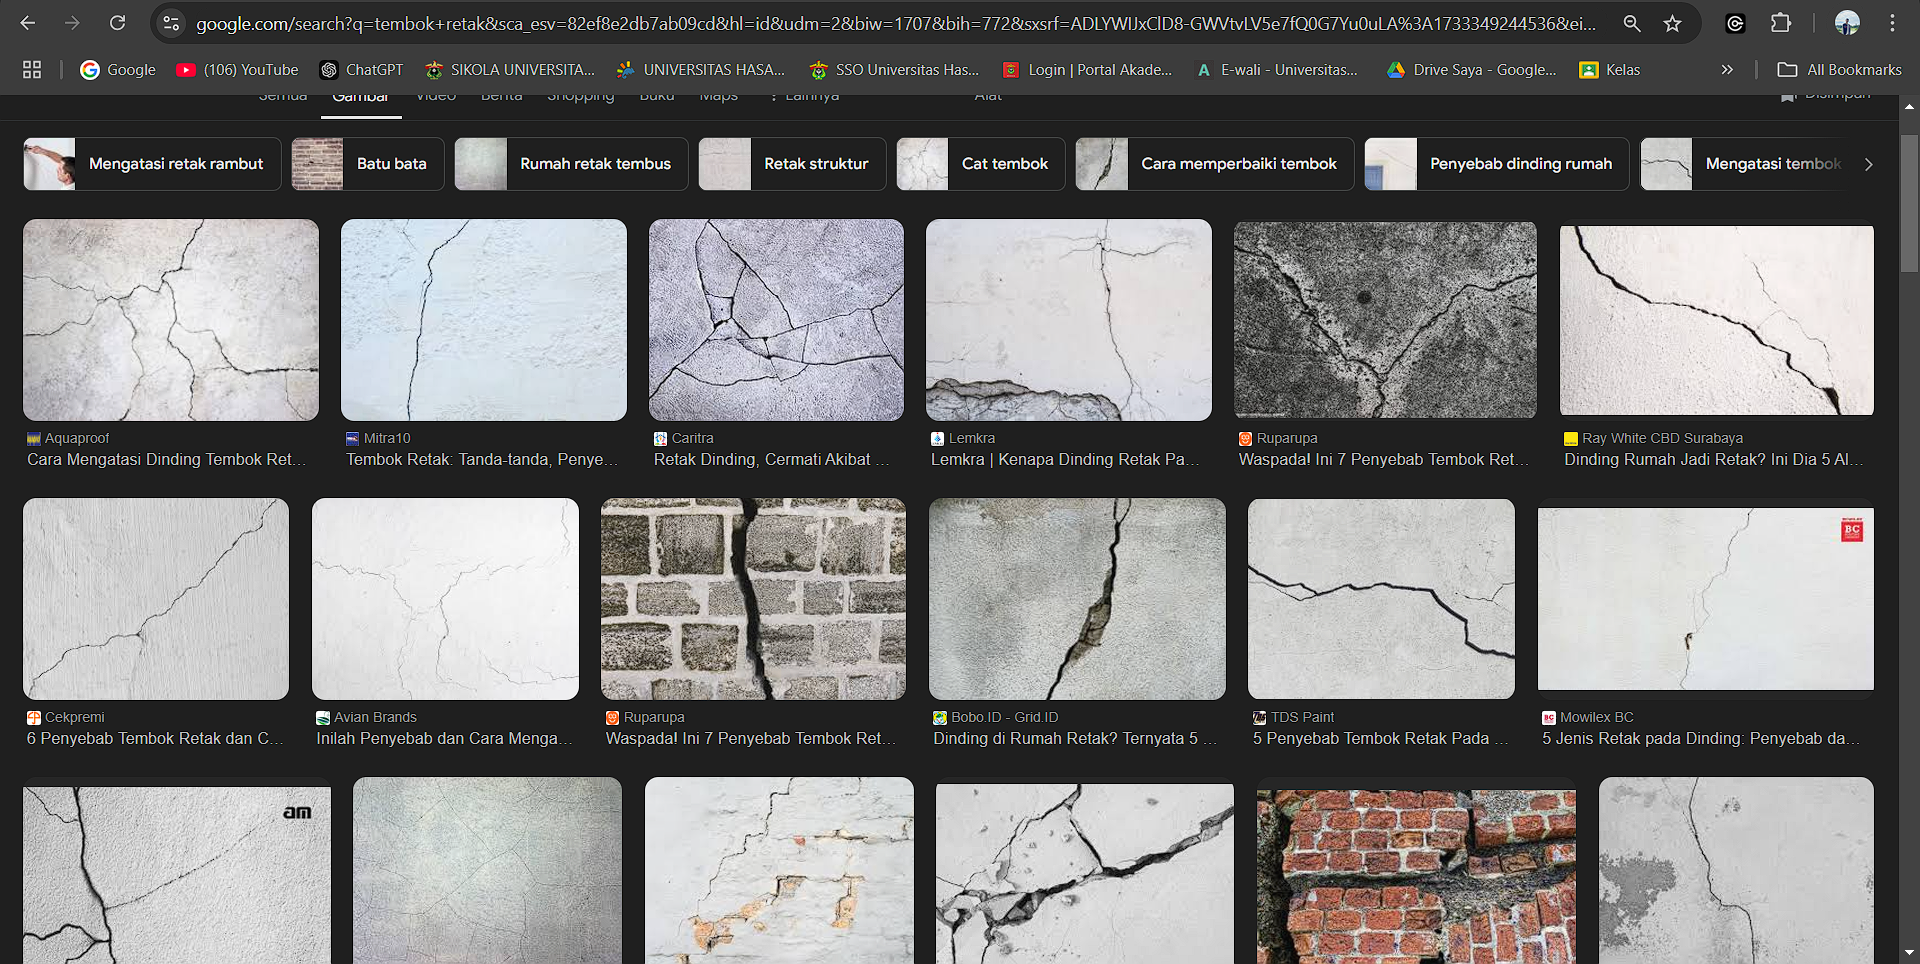
\includegraphics[width=0.8\linewidth]{google.png}
        \caption*{Gambar 2. Pengambilan Gambar Di Google Images}
        \label{fig:enter-label}
    \end{figure}
    \begin{figure}[H]
        \centering
        \label{fig:enter-label}
    \end{figure}
\end{itemize}


% 4. Result and Discussion
\section{Result and Discussion}
Hasil penelitian ini menunjukkan bahwa penggunaan model Inception dalam klasifikasi  memiliki akurasi prediksi yang memuaskan dengan angka 74\% dan indikasi overfitting kecil. Setiap model ditrain dengan 20 epoch, masing-masing memiliki 50 step per epoch. Pada awalnya, setiap model ditrain tanpa adanya optimisasi yang perlu. Model Inception mencapai 50\% akurasi pada epoch pertama, lebih tinggi dibandingkan ResNet yang mencapai 19\% dan model CNN biasa yang memiliki akurasi 32\%. Akurasi akhir dari Inception, CNN, dan ResNet secara berturut-turut adalah 96\%, 85\% dan 42\%. Perbandingan akurasi dan loss dari ketiga model adalah sebagai berikut:

\begin{itemize}
    \item Inception
    \begin{figure}[H]
        \centering
       \includegraphics[width=0.8\textwidth]{Incept 1.png}
        \caption*{Gambar 3. Akurasi dan loss awal pada Inception}
        \label{fig:enter-label}
    \end{figure}
\end{itemize}
\begin{itemize}
    \item CNN
    \begin{figure}[H]
        \centering
       \includegraphics[width=0.8\textwidth]{CNN 1.png}
        \caption*{Gambar 4. Akurasi dan loss awal pada CNN}
        \label{fig:enter-label}
    \end{figure}
\end{itemize}
\begin{itemize}
    \item ResNet
    \begin{figure}[H]
        \centering
       \includegraphics[width=0.8\textwidth]{Resnet 1.png}
        \caption*{Gambar 5. Akurasi dan loss awal pada ResNet}
        \label{fig:enter-label}
    \end{figure}
\end{itemize}
Model Inception memiliki perbedaan signifikan pada akurasi train dan validasi, mengindikasikan adanya overfitting. Disisi lain terdapat kesenjangan pada akurasi dan loss pada train dan validasi di CNN yang juga mengindikasikan adanya overfitting, dikarenakan model mampu untuk mengklasifikasikan data train, namun gagal untuk mengklasifikasikan data validasi secara akurat. Sebaliknya model ResNet mengalami underfitting, hal ini diindikasikan dari akurasi yang cukup rendah dan model loss yang bernilai lebih dari satu.

Berikut adalah grafik  Receiver Operating Characteristic (ROC) dari ketiga model :
\begin{itemize}
    \item Inception
    \begin{figure}[H]
        \centering
       \includegraphics[width=0.8\textwidth]{Incep-ROC 1.png}
        \caption*{Gambar 6. ROC awal pada Inception}
        \label{fig:enter-label}
    \end{figure}
\end{itemize}
\begin{itemize}
    \item CNN
    \begin{figure}[H]
        \centering
       \includegraphics[width=0.8\textwidth]{CNN ROC 1.png}
        \caption*{Gambar 7. ROC awal pada CNN}
        \label{fig:enter-label}
    \end{figure}
\end{itemize}
\begin{itemize}
    \item ResNet
    \begin{figure}[H]
        \centering
       \includegraphics[width=0.8\textwidth]{Resnet ROC 1.png}
        \caption*{Gambar 8. ROC awal pada ResNet}
        \label{fig:enter-label}
    \end{figure}
\end{itemize}
Dari ketiga model diatas, kita dapat menyimpulkan bahwa model inception memiliki performa yang paling baik, namun karena terdapat indikasi overfitting, sehingga grafik ROC menjadi kurang valid. Dari grafik ROC kelas 2 (minimalisme) memiliki akurasi yang cukup tinggi, hal ini mengimplikasikan bahwa kelas minimalisme memiliki perbedaan fitur yang mampu membedakannya dengan kelas lain.



\noindent Dari hasil train diatas, dapat dilakukan beberapa optimisasi untuk menaikkan akurasi model dan meminimalisir overfitting, metode yang dilakukan yakni generalisation dan fine tuning.

\subsection{Generalisasi}
Generalisasi adalah kemampuan suatu model untuk memberikan prediksi akurat terhadap data baru yang tidak digunakan selama proses pelatihan. Karena tujuan utama pengembangan model pembelajaran mesin adalah untuk memaksimalkan akurasi tidak hanya pada data pelatihan tetapi juga pada data yang belum pernah dilihat sebelumnya, generalisasi penting saat mengevaluasi kinerja model. 

Laporan ini mengukur generalisasi dengan membandingkan metrik kinerja seperti akurasi, kerugian, dan AUC-ROC antara data pelatihan, validasi, dan pengujian. Suatu model dianggap \textit{overfitted} jika performa model pada data pelatihan jauh lebih baik dibandingkan pada data validasi atau pengujian. Hal ini menunjukkan bahwa model terlalu spesifik terhadap pola dalam data pelatihan dan gagal menangkap pola yang lebih umum.

\begin{figure}[h]
    \captionsetup{labelformat=empty}
    \centering
    \includegraphics[width=0.8\textwidth]{Generalization.png} % Ganti dengan nama file gambar Anda
    \caption{Gambar 9. Generalisasi model pada data pelatihan, validasi, dan pengujian.}
    \label{fig:generalization}
\end{figure}
\subsection{Fine Tuning}
Fine-tuning adalah proses penyesuaian ulang parameter model dengan tujuan meningkatkan performa dan kemampuan generalisasi pada dataset tertentu. Proses ini dilakukan terutama pada model yang telah dilatih sebelumnya (\textit{pre-trained model}), di mana bobot awal model digunakan sebagai titik awal, kemudian disesuaikan dengan data spesifik yang sedang ditangani. 

Fine-tuning memungkinkan model untuk memanfaatkan pengetahuan umum yang diperoleh dari dataset besar, seperti pola dasar dalam gambar atau teks, sekaligus beradaptasi dengan karakteristik unik dataset target. Dalam proyek ini, \textit{fine-tuning} dilakukan dengan memanipulasi \textit{learning rate} menjadi 0.001 dan membekukan semua \textit{layer} jaringan neural kecuali 50 \textit{layer} terakhir.

\begin{figure}[h]
    \captionsetup{labelformat=empty} 
    \centering
    \includegraphics[width=0.8\textwidth]{Fine Tuning.png} % Ganti dengan nama file gambar Anda
    \caption{Gambar 10. Proses fine-tuning model pada dataset spesifik.}
    \label{fig:fine_tuning}
\end{figure}

Setelah dilakukan optimisasi, pelatihan kembali dilakukan untuk mengevaluasi model. Hasilnya, model Inception memiliki akurasi 74\%, CNN mencapai 55\%, dan ResNet mencapai 51\%. Grafik perbandingan hasil akurasi model adalah sebagai berikut:
\begin{itemize}
    \item Inception
    \begin{figure}[H]
        \centering
       \includegraphics[width=0.8\textwidth]{Incept 2.png}
        \caption*{Gambar 11. Akurasi dan loss pada Inception}
        \label{fig:enter-label}
    \end{figure}
\end{itemize}
\begin{itemize}
    \item CNN
    \begin{figure}[H]
        \centering
       \includegraphics[width=0.8\textwidth]{CNN 2.png}
        \caption*{Gambar 12. Akurasi dan loss pada CNN}
        \label{fig:enter-label}
    \end{figure}
\end{itemize}
\begin{itemize}
    \item ResNet
    \begin{figure}[H]
        \centering
       \includegraphics[width=0.8\textwidth]{Resnet 2.png}
        \caption*{Gambar 13. Akurasi dan loss pada ResNet}
        \label{fig:enter-label}
    \end{figure}
\end{itemize}
Dari ketiga grafik diatas, model Inception memiliki performa paling baik dengan akurasi dan loss yang tidak begitu fluktuatif. Model CNN mengalami fluktuasi pada validasi yang mengindikasikan model mengalami kendala dalam generalisasi data validasi. ResNet mengalami fluktuasi pada akurasi, hal ini bisa terjadi karena model yang terlalu kompleks atau learning rate yang terlalu tinggi. Kedua hal ini mengindikasikan overfitting pada model CNN dan ResNet.
Grafik ROC seperti berikut:
\begin{itemize}
    \item Inception
    \begin{figure}[H]
        \centering
       \includegraphics[width=0.8\textwidth]{Incept2ROC-2.png}
        \caption*{Gambar 14 . ROC  pada Inception}
        \label{fig:enter-label}
    \end{figure}
\end{itemize}
\begin{itemize}
    \item CNN
    \begin{figure}[H]
        \centering
       \includegraphics[width=0.8\textwidth]{CNN ROC 2.png}
        \caption*{Gambar 15 . ROC  pada CNN}
        \label{fig:enter-label}
    \end{figure}
\end{itemize}
\begin{itemize}
    \item ResNet
    \begin{figure}[H]
        \centering
       \includegraphics[width=0.8\textwidth]{Resnet ROC 2.png}
        \caption*{Gambar 16 . ROC  pada ResNet}
        \label{fig:enter-label}
    \end{figure}
\end{itemize}


Hasilnya, model Inception memiliki akurasi yang paling tinggi dan stabil dibandingkan model yang lain. Namun perlu diperhatikan bahwa model Inception masih belum optimal akibat akurasinya yang masih dibawah 80\%, hal ini bisa disebabkan oleh kurangnya dataset yang diberikan pada model. 

\subsection{Confusion Matrix}

Confusion matrix adalah alat evaluasi kinerja model klasifikasi yang memberikan gambaran detail tentang prediksi model dibandingkan dengan label yang sebenarnya. Matriks ini terdiri dari empat elemen utama untuk setiap kelas dalam dataset:

True Positive (TP): Jumlah sampel yang benar-benar termasuk dalam kelas tertentu dan berhasil diprediksi dengan benar oleh model.
False Positive (FP): Jumlah sampel yang sebenarnya bukan dari kelas tertentu tetapi diprediksi sebagai kelas tersebut oleh model.
False Negative (FN): Jumlah sampel yang sebenarnya dari kelas tertentu tetapi tidak diprediksi sebagai kelas tersebut oleh model.
True Negative (TN): Jumlah sampel yang bukan dari kelas tertentu dan tidak diprediksi sebagai kelas tersebut oleh model.
\begin{itemize}
    \item Inception
    \begin{figure}[H]
        \centering
       \includegraphics[width=0.8\textwidth]{Inc CF.png}
        \caption*{Gambar 17 . Confusion Matrix  pada Inception}
        \label{fig:enter-label}
    \end{figure}
\end{itemize}
\begin{itemize}
    \item CNN
    \begin{figure}[H]
        \centering
       \includegraphics[width=0.8\textwidth]{CNN CF.png}
        \caption*{Gambar 18 . Confusion Matrix pada CNN}
        \label{fig:enter-label}
    \end{figure}
\end{itemize}
\begin{itemize}
    \item ResNet
    \begin{figure}[H]
        \centering
       \includegraphics[width=0.8\textwidth]{ResNet CF.png}
        \caption*{Gambar 19 . Confusion Matrix pada ResNet}
        \label{fig:enter-label}
    \end{figure}
\end{itemize}
Berdasarkan ketiga grafik confusion matrix yang disajikan, dapat disimpulkan sebagai berikut:

Gambar 17 memperlihatkan hasil model Inception, yang menunjukkan bahwa model ini sudah mampu membedakan kelas 'abstrak', 'kubisme', dan 'surealisme' dengan baik. Namun, model Inception masih mengalami kesulitan dalam membedakan kelas 'minimalism' dari kelas lainnya.

Gambar 18 menampilkan hasil model CNN dengan layer manual, di mana terdapat peningkatan performa dalam membedakan kelas 'abstrak' dan 'kubisme' dibandingkan model ResNet. Akan tetapi, model CNN masih kesulitan dalam membedakan kelas 'minimalism' dan 'surealisme'.

Gambar 19 menunjukkan bahwa model ResNet memiliki kinerja terbaik dalam mengidentifikasi kelas 'surealisme' dengan persentase klasifikasi benar (true positive) sebesar 81\%. Namun, model ini masih mengalami kesulitan dalam membedakan kelas 'abstrak' dan 'kubisme', dengan banyak terjadi kesalahan klasifikasi antar kedua kelas tersebut.

Secara keseluruhan, ketiga model menunjukkan performa yang beragam dalam mengklasifikasikan karya seni ke dalam kategori 'abstrak', 'kubisme', 'minimalism', dan 'surealisme'. Performa terbaik terlihat pada kelas 'surealisme', sementara kelas 'minimalism' tampak menjadi yang paling sulit dibedakan oleh semua model. 
Hasilnya, dapat disimpulkan bahwa model Inception memiliki banyak prediksi yang True Positive atau prediksinya benar


% 5. Conclusion
\section{Conclusion}
Proyek ini bertujuan untuk membandingkan model untuk klasifikasi lukisan pada 4 tipe lukisan dengan menggunakan model CNN, Resnet, dan Inception. Hasil menunjukkan bahwa model Inception memiliki performa yang cukup meyakinkan dengan akurasi akhir 74\% dan loss 65\% serta rendahnya indikasi overfitting. Hal ini juga diperkuat dengan perbandingan confusion matrix
Proyek ini menunjukkan pentingnya pemilihan model yang sesuai dalam membuat suatu perangkat klasifikasi. Model Inception mampu belajar dengan optimal walau ukuran dataset kecil. Sebaliknya model ResNet membutuhkan dataset yang lebih banyak untuk menghasilkan output yang lebih baik. Sehingga mempunyai dataset yang besar untuk melatih model juga mempunyai pengaruh signifikan pada pembuatan algoritma klasifikasi.

\newpage

\begin{thebibliography}{9}

\bibitem{yogieeka2611} 
Yogie Eka Pratama, 
"Pengembangan Aplikasi Pembelajaran Mesin untuk Identifikasi Kemiripan Lukisan," 
\textit{Institut Teknologi dan Bisnis Kalbis},
Vol. 9, No. 4, 2023.


\end{thebibliography}

\end{document}